\label{desenvolvimento_eletroeletronica}

Nesta seção é descrito o detalhamento da solução do módulo de eletroeletrônica, resultante das duas primeiras fases, 
e o seu projeto e construção, resultante da Fase 03.

\subsection{Detalhamento da Solução}

  \subsubsection*{\textbf{Sensoriamento e disponibilização dos dados}}
  \subsubsubsection*{Requisito}
  Uma mesa de vibração necessita detalhes específicos sobre as forças que estão sendo aplicadas no decorrer do experimento. 
  Na prática, isso implica em uma grande oferta de sensores capazes de cumprir com taxas de amostragem altas. A frequência na 
  qual os sensores devem amostrar os dados pode ser estimada utilizando o teorema de \textit{Nyquist-Shannon}, que estabelece 
  que frequências de amostragem em sinais contínuos devem ser pelo menos maiores que o dobro da sua frequência. Trazendo isso 
  para o escopo do projeto, que funciona de 50 a 100Hz, teremos no pior caso que amostrar a base à no mínimo 200Hz. Com leituras
  contínuas nessa velocidade, evitamos o efeito \textit{Aliasing}, que é a perda do formato da onda devido a baixa amostragem.
  Também cabe dizer que quanto mais próximo de um movimento senoidal de frequência única, melhor. Isso pois o processo acaba sendo
  melhor modelado em alguns parâmetros bem definidos: Amplitude, Frequência, Velocidade e Aceleração. Mas, em todo caso, frequências 
  de ordens superiores ainda podem estar presentes, inviabilizando a obtenção da leitura. Nesse caso, a estrutura deve ser preenchida
  por filtros passa-baixas passivos que atuem de forma a eliminar estes problemas.Por fim, o alvo dos testes, seja uma estrutura, 
  seja um outro dispositivo, também necessita ser validado em alguns aspectos. Primeiro, o seu peso não pode ultrapassar o limite 
  seguro para a estrutura começar a rotina de testes, do contrário há muita propensão a acidentes ou a danos estruturais à bancada. 
  Da mesma forma, deve-se ter o \textit{feedback} de alguns pontos chaves do objeto medido, para se ter ideia da vibração no corpo a 
  ser medido.
  \subsubsubsection*{Implementação}
Optou-se por um esquema de barramento para obter dados de sensores, pois há a facilidade de conectar uma 
grande quantidade deles e compartilhar a mesma rede. Neste caso, optou-se pela rede I2C (\textit{Inter Intergrated Circuits}),
onde todos os periféricos recebem 2 sinais de comunicação (Sinal de dados ou \textit{SDA} e Sinal de \textit{clock}, ou \textit{SCL}). A solução permite ter diversos sensores individuais sem a necessidade de um aumento de infraestrutura. Para garantir que a taxa de amostragem do sistema esteja dentro dos requisitos expostos anteriormente, será utilizado um microcontrolador dedicado para essa tarefa. Para a identificação da vibração na mesa foram escolhidos sensores do tipo Acelerômetros. Estes são especialmente desenvolvidos para aferir aceleração em eixos distintos.

\subsubsubsection*{Como acelerômetros funcionam}
Grande parte dos acelerômetros trabalham a partir dos princípios dos efeitos piezoelétricos, 
que ocorrem quando cristais são excitados e consequentemente geram uma diferencia de potencial elétrico.  
Acelerômetros piezoelétricos trabalham usando a segunda lei de newton (\textit{Força = Massa X Aceleração}). A
aceleração do objeto em questão a ser avaliado é transmitida para uma massa sísmica dentro do acelerômetro, essa massa 
gera uma forca proporcional em um cristal piezoelétrico que consequentemente gera uma tensão elétrica proporcional a aceleração.
Resumindo, a massa converte a aceleração a ser medida em uma forca, e o cristal converte essa forca em uma tensão elétrica que 
indica a aceleração em questão. 

\subsubsubsection*{Parâmetros importantes de serem avaliados na escolha de um acelerômetro}
\begin{itemize}
\item Amplitude de vibração: Se a amplitude de vibração for superior a especificação do acelerômetro o mesmo ira grampear o sinal de saída ou ate provocar uma distorção. Geralmente o aumento da amplitude resulta em uma menor sensibilidade para o sensor.
\item Sensibilidade: Talvez o parâmetro mais importante, descreve a conversão entre vibração e tensão elétrica, geralmente é dada por \textit{mV/G} (onde \textit{G} é a aceleração da terra, 9.81 $m/s^2$ ). A sensibilidade de um sensor de aceleração também é afetada pela frequência de vibração, o dispositivo é apto a operar dentro de um intervalo de frequência determinado pelo fabricante.
\item Frequência de Vibração: Como citado anteriormente, os sensores de aceleração possuem intervalos de frequência que estão aptos a operar. Se essa frequência for muito baixa é possível que o equipamento nem a detecte e se for muito alta é provável que a tensão de saída sature ou até mesmo que o sensor seja danificado.
\item Numero de eixos: Os tipos mais simples de acelerômetros são uniaxiais, isto é, medem a aceleração para um único eixo orientado dependendo da maneira com que o acelerômetro esta montado na estrutura. Existem também acelerômetros biaxiais e triaxiais, os acelerômetros triaxiais geram três sinais tensão que geralmente são usados para determinar o tipo de vibração seja ela lateral, transversal ou rotacional.
\end{itemize}

\subsubsubsection*{Medições com acelerômetros}
\begin{itemize}
  \item Aceleração e amplitude de vibração: Naturalmente dadas pela tensão elétrica gerada na saída do sensor, porem costuma-se ser mais usado o valor \textit{RMS} (\textit{Root Mean Square}) do sinal para que uma noção melhor da energia de vibração possa ser interpretada.
  \item Velocidade: Sabendo que a velocidade pode ser calculada pela integral da aceleração, para extrair a velocidade de vibração de um sistema/estrutura em questão a solução consiste em integrar o sinal de aceleração e assim obter a velocidade.
  \item Deslocamento: Conhecer o quanto que uma estrutura se desloca enquanto vibra é um parâmetro muito importante em uma analise vibratória. Sabe-se que o deslocamento em função do tempo é dado pela dupla derivada da aceleração no tempo, assim usando o parâmetro de aceleração que o acelerômetro nos da se torna possível analisar o deslocamento da estrutura.
  \item Frequência: É um parâmetro que pode ser difícil de ser analisado pois depende que a vibração com qual a estrutura é excitada seja próxima de constante durante um breve período de tempo, quanto maior esse intervalo de tempo maior sera a precisão dessa medição. A frequência costuma ser obtida atraves de algorítimos de processamento do sinal de aceleração.
\end{itemize}

\subsubsection*{Controle de Malha Fechada}
\subsubsubsection*{Requisito}
\begin{figure}[H]
\centering
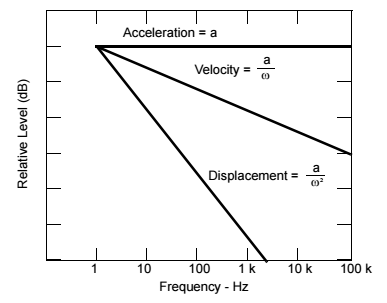
\includegraphics[scale=0.5]{figuras/imagem1_eletro.png}
\caption{Sinais do Acelerômetro.  Fonte: Autores}
\label{fig:signal_acel}
\end{figure}
É importante que o sistema seja capaz de garantir que os parâmetros de vibração inseridos pelo usuário em camadas superiores do 
sistema sejam efetivamente o que acontece fisicamente, para implementar essa funcionalidade será usado um sistema de controle por
malha fechada. Esse procedimento pode ser representado pela imagem abaixo:
\begin{figure}[H]
\centering
\includegraphics[scale=0.3]{figuras/imagem4_eletro.png}
\caption{Sistema de Controle por Malha Fechada.  Fonte: Autores}
\label{fig:malha_fecha}
\end{figure}
O que sistema de controle eletroeletrônico faz é receber um valor de frequência das camadas superiores de interface/processamento 
e converter essa informação em sinais elétricos. Esses sinais elétricos serviram para controlar o mecanismo vibrador que irá excitar 
a plataforma vibratória. Na plataforma vibratória existiram sensores que iram informar ao sistema de controle qual a vibração que os 
sinais elétricos estão provocando. O sistema de controle deverá através desse sinal de retorno avaliar se os sinais elétricos que o 
mesmo está produzindo estão coerentes com o que o sistema de Interface/Processamento lhe informou anteriormente. O mecanismo vibrador 
será constituído por um inversor de frequência que controla a velocidade de um motor trifásico que irá através de um sistema mecânico 
provocar a vibração na mesa. A programação do inversor de frequência e o controle do motor não é realizado pelo sistema 
eletroeletrônico, o sistema apenas fornece níveis de tensão analógica e sinais digitais para informar o inversor a velocidade com 
qual o motor deve vibrar.
\subsubsubsection*{Implementação}
A figura a seguir ilustra como será o sistema eletrônico planejado para o controle em frequência. No projeto, existem 2 
microcontroladores atuando em conjunto. O primeiro, e principal, é o MCU 1. Ele garante algumas coisas no sistema:
\begin{enumerate}
\item Velocidade de amostragem correta
\item Comunicação com \textit{Raspberry Pi} via \textit{UART}
\item Comunicação com a interface do motor via \textit{$I_{2} C$}
\end{enumerate}
A segunda parte do projeto é a MCU2, responsável pela manutenção do requisito de vibração na mesa. A partir das 
informações contidas no barramento, a mesma irá aumentar ou diminuir a velocidade dos motores (a partir de uma interface 
analógica com o motor), atuando como um controlador PI. As informações como frequência almejada, velocidade atual e 
frequência atual serão enviadas compartilhadas pelo barramento.
\begin{figure}[H]
\centering
\includegraphics[scale=0.15]{figuras/imagem5_eletro.png}
\caption{Detalhamento do Sistema de Controle. Fonte: Autores}
\label{fig:det_control_system}
\end{figure}

\subsection{Projeto e Construção}

% COLOCAR AQUI TEXTO DO PC2